\documentclass[tikz,border=3mm]{standalone}
\usepackage{tikzlings}
\newcounter{Sunday}
\usetikzlibrary{positioning,calendar,backgrounds}
\renewcommand\familydefault\sfdefault
\colorlet{darkgreen}{green!50!black}
\colorlet{holiday}{black!50}
\newcommand{\calrow}[1]{\node[anchor=base east](Mon){M};
\node[base right=of Mon](Tue){T}; \node[base right=of Tue](Wed){W};
\node[base right=of Wed](Thu){T}; \node[base right=of Thu](Fri){F};
\node[base right=of Fri](Sat){S}; \node[base right=of Sat](Sun){S};
\node[darkgreen, above=of Thu]{\textbf{#1}};}

\newcommand{\calperiod}[2][\currentyear]{%
  \calendar[dates=\currentyear-#2-01 to \currentyear-#2-last,
  execute at begin day scope={\ifdate{Sunday}{\stepcounter{Sunday}
   \node[anchor=base east] (SD-\number\value{Sunday}){};}}]
    if (Sunday) [holiday] \holidays;}
\edef\currentyear{\the\year}
\newcommand{\holidays}{% 
if (equals=01-01) [holiday]%
if (equals=01-06) [holiday]%
if (equals=05-01) [holiday]%
if (equals=08-15) [holiday]%
if (equals=11-01) [holiday]%
if (equals=12-06) [holiday]%
if (equals=12-25) [holiday]%
if (equals=12-26) [holiday]%
}

\newcommand*\circled[1]{\tikz[baseline=(char.base)]{
            \node[shape=circle,draw,inner sep=2pt,fill=white,circular glow={fill=rdsColor!40!white},thin] (char) {#1};}}

\tikzset{tikzling/.style={execute at begin day scope={\typeout{X}}}}
\begin{document}
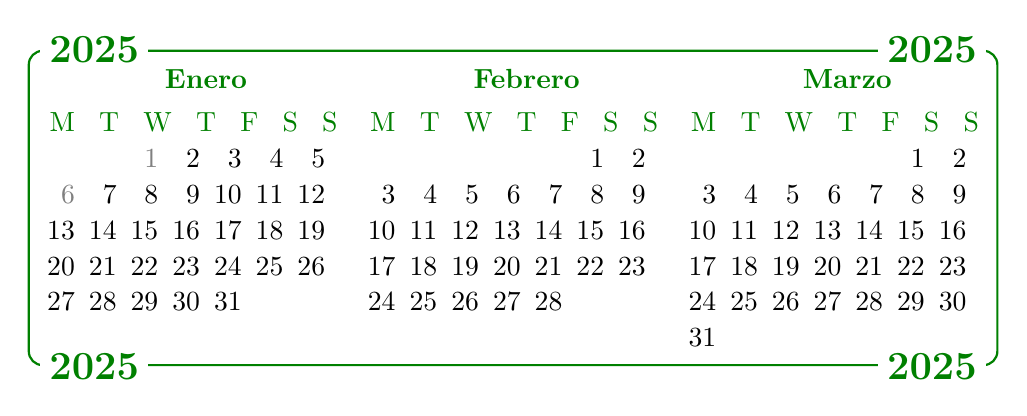
\begin{tikzpicture}[every calendar/.style={week list},
year label/.style={
  fill=white,text=darkgreen,font=\bfseries\Large
}, current year/.store in=\currentyear,
current year=2025]
\matrix[%
row 1/.style={darkgreen,node distance=.3ex},%
row 3/.style={darkgreen,node distance=.3ex},
row 5/.style={darkgreen,node distance=.3ex},
row 7/.style={darkgreen,node distance=.3ex},
column sep=1ex,%
draw=darkgreen,thick,rounded corners=5pt,%
append after command={ 
  \pgfextra{\edef\matrixname{\tikzlastnode}}
  node [year label/.try, right=1ex of \matrixname.south west] {\currentyear}
  node [year label/.try, right=1ex of \matrixname.north west] {\currentyear}
  node [year label/.try, left=1ex of \matrixname.south east] {\currentyear}
  node [year label/.try, left=1ex of \matrixname.north east] {\currentyear}
}
]{%

% first row: week day and month
\calrow{Enero} & \calrow{Febrero} & \calrow{Marzo} \\
\calperiod{01} & \calperiod{02} & \calperiod{03} \\[1ex]
% % second row: calendar
% \calrow{Abril} & \calrow{Mayo} & \calrow{Junio} \\
% \calperiod{04} & \calperiod{05} & \calperiod{06} \\[1ex]
% % third row: week day and month
% \calrow{Julio} & \calrow{Agosto} & \calrow{Septiembre} \\
% \calperiod{07} & \calperiod{08} & \calperiod{09} \\[1ex]
% % forth row: calendar
% \calrow{Octubre} & \calrow{Noviembre} & \calrow{Diciembre} \\
% \calperiod{10} & \calperiod{11} & \calperiod{12} \\[1ex]\\
};

\end{tikzpicture}
\end{document}